\chapter{The Uncanny Curve}
In Masahiro Mori's original hypothesis \cite{original_masahiro}, one can see that if the appearance and the movements of an entity become indistinguishable from humans it is possible for the entity to escape the uncanny valley. Moreover it is even possible that the affinity for an entity, which has overcome the uncanny valley, exceeds the affinity of entities which have not yet fallen into the uncanny valley. If this hypotheses holds true, it would have major implications for robotics and other scientific fields as they must strive to design entities whose looks and movements are as similar as possible to that of a human being.\\
On the contrary it may be possible that the uncanny valley  is not as clearly defined as Masahiro Mori suggests and that it could resemble an uncanny cliff or even an uncanny wall in which the affinity towards entities with perfect or near perfect human likeness is in general lower than that of entities that did not fall into the uncanny valley. In these hypotheses, it may not be advantageous to strive for perfect human likeness.

\section{A Hazy Uncanny Valley}
Masahiro Mori has proposed the uncanny valley as a well-defined graph with a clearly visible dip in affinity as human likeness increases. Furthermore movement merely steepens the slopes of the uncanny valley in his proposal.
In one of his studies, MacDorman \cite{uncanny_ambiguous} investigated whether the uncanny valley is as clearly defined as Masahiro Mori suggests. To further observe whether human likeness is the main triggering factor, he focused on using androids and robots as stimuli, performing a variety of activities in different environments. For his study he recruited 56 Indonesian participants, 43 male and 13 female, of whom 13 were 17 to 20 years old, 36 were 21 to 25, 4 were 26 to 30, and 3 were 31 to 35. Having been recruited in an internet cafe and being mostly  university students, young professionals, and government workers, the participants had extensive technical experience.\newpage
\begin{wrapfigure}[25]{r}{0.5\textwidth} %this figure will be at the right
    \centering
    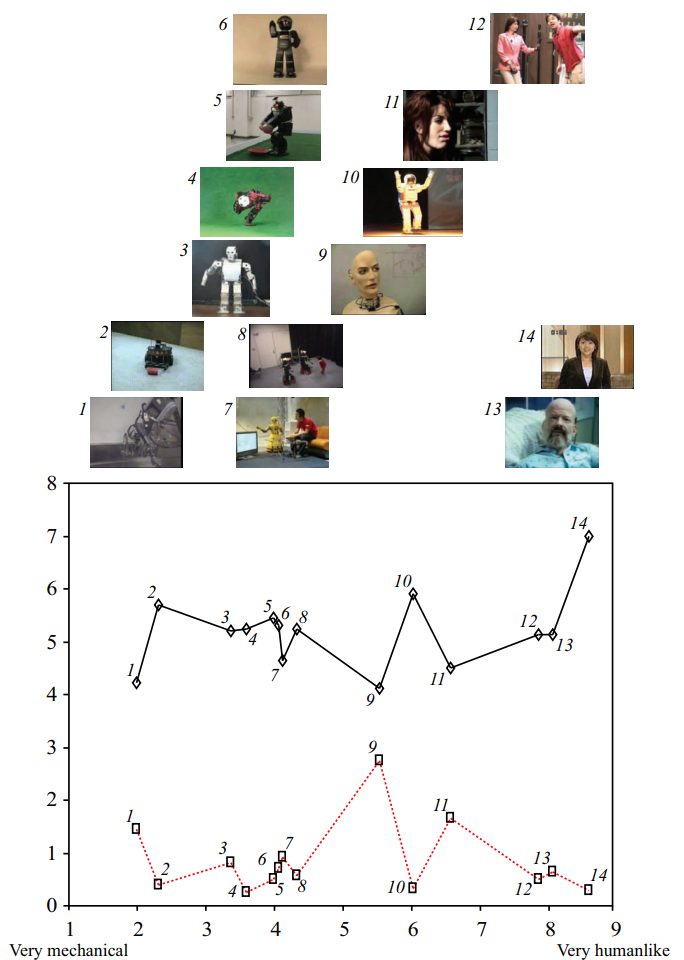
\includegraphics[width=0.5\textwidth]{graphics/hazy_uncanny.png}
    \caption{Result graph of the ratings for the 14 videos.}
    \label{fig:hazyUncanny}
\end{wrapfigure}
The study procedure consisted of a questionnaire in which the participants had to rate 14 video clips, which were 30 to 60 seconds in length, on a nine-point mechanical versus humanlike scale, a nine-point strange versus familiar scale, and a
ten-point eeriness scale. A main focus was placed on the selected videos, which consisted of  mobile robot (Pioneer II), a manipulator arm, seven humanoid robots (Rovovie-M3, HR-2, VisiON Nexta, Chronio, Robovie, Wakamaru, Asimo), two android heads (K-bot, Eva), two androids (Philip K. Dick, Repliee Q1Expo), and one human being. The entities depicted in the videos performed different actions in different contexts, sometimes also with speech accompaniment.\\
Figure \ref{fig:hazyUncanny} shows the videos used together with the evaluations of the questionnaire. The solid line plots the relationship between perceived human likeness and perceived familiarity. The dashed line plots the relationship between
perceived human likeness and eeriness. The results of his study show that there is not one particular uncanny valley for a particular range of human likeness. The study therefore concludes that human likeness is only one of many factors influencing the extent of the uncanny valley effect.\\
From this study, one can conclude that in the real world scenarios with many different influences and situations in which one might encounter the uncanny valley,  it may not only be triggered by the appearance of an entity alone but by many different influences in the respective situation. This creates a much more difficult picture of the uncanny valley than Masahiro Mori suggested. However, the question of whether it is possible to overcome the uncanny valley remains open in this study.

\section{An Uncanny Cliff}
A study by Bartneck et al. \cite{uncanny_cliff}, tried to plot the uncanny valley with particular emphasis on the last ascending section of the curve. Furthermore, the referred study also dealt with the question whether highly humanlike androids are perceived more likeable when they are being framed as robots.\\
In this study a framing and a anthropomorphism experiment were conducted. Framing contained three conditions: human, robot and none. Anthropomorphism consisted of four conditions real human, manipulated human, computer graphic and android. Additionally only in the robot framing condition two additional anthropomorphisms were present: humanoid and pet robot. For the experiment only pictures of entities that either exist or which are extremely similar to existing entities were chosen. 
With a questionnaire the human likeness and the likeability of the stimuli was measured.
To ensure the framing conditions of this study, three different questionnaires with different framings of the pictures where created. In each different framing the pictures were either framed as human, robot or only as a face for a neutral comparison. For each anthropomorphism category three different pictures where shown to the participants. 
58 people participated in the study aged between 18 and 41 years. 28 of which were female and 30 were male.
Each of the 18 chosen stimuli was presented to the participants twice. Once with a question about the liking towards the entity, which could be rated on a scale form one to seven and once with a 7-point semantic differential scales consisting of the values fake/natural, machinelike/humanlike, unconscious/conscious, artificial/lifelike, nice/awful, friendly/unfriendly, kind/unkind, and pleasant/unpleasant. This resulted in 36 questions which the participants had to answer on a computer in an randomized order.\\
This study came to the conclusion that the framing of the entities had no significant influence on the measurements. The pictures where evaluated independently from weather they were labeled as human, robot or face and the labeling did not impact the likeability or human likeness in a negative or positive way.
However the results of the questionnaire showed that anthropomorphism had significant influence on human likeness and likeability. The participants most liked the pictures of toy robots and humanoids. Even though a small upwards trend in likability towards highly humanlike entities was noted, not even the pictures of humans reached the affection level of the pictures of toy robots. On the basis of these results the study speculates that even the most humanlike androids are not liked as much as toy robots or humanoid. Therefore the study suggests a revised graph of Mori's original graph where there may be small valleys but the main feature is a cliff which is depicted in figure \ref{fig:uncannyCliff}.
\begin{wrapfigure}[13]{r}{0.5\textwidth} %this figure will be at the right
    \centering
    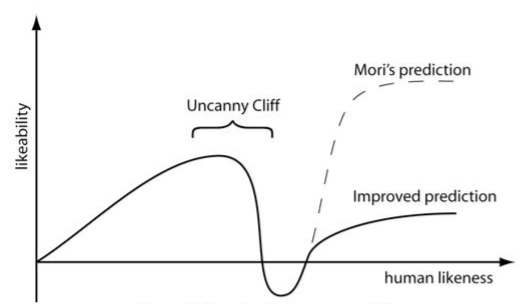
\includegraphics[width=0.5\textwidth]{graphics/uncanny_cliff.png}
    \caption{Hypothesized uncanny cliff.}
    \label{fig:uncannyCliff}
\end{wrapfigure}
In summary, the figure \ref{fig:uncannyCliff} would therefore not describe an uncanny valley but an uncanny cliff.
The results of this study would imply that it is unwise to attempt to build highly humanlike entities, since a machinelike robot would be liked more. However, the study mentions that in order to further test the hypothesis, more studies need to be conducted with participants from different cultures, as the group of participants in the presented study consisted only of Japanese people, who are stereotypically thought of as being more avid robot-aficionados than other cultures.

\section{An Uncanny Wall}
Both in robotics and in the creation of virtual characters for films and other media, ever-improving technology is allowing progress to be made towards increasing realism. On the basis of these improvements Angela Tinwell and Mark Grimshaw \cite{uncanny_wall} designed a study to furthermore examine and plot the curve of the uncanny valley by using videos of virtual characters.\\
For the study Tinwell et al. choose 100 participants, 92 of them where males and eight females, who where mainly university students from the creative technology field and professionals working within this academic sector and the video game industry. The selected focus group for the study therefore consisted exclusively of people with a lot of knowledge about informatics and game design and art and therefore a lot of exposure and comprehension about the the uncanny valley. Furthermore, significantly more men were selected for the study and no information was given about their age. 
\begin{wrapfigure}[16]{r}{0.6\textwidth} %this figure will be at the right
    \centering
    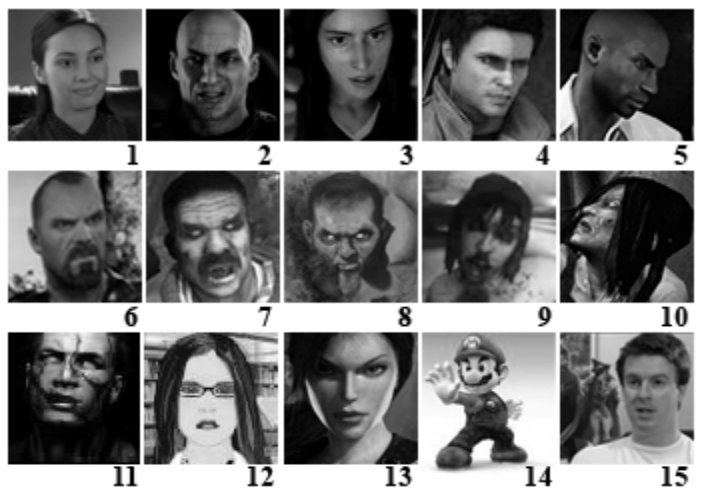
\includegraphics[width=0.6\textwidth]{graphics/uncanny_wall.png}
    \caption{The 15 characters chosen for the study.}
    \label{fig:uncannyWall}
\end{wrapfigure}
The method of the study consisted of a web based questionnaire in which the participants had to rate 14 video clips of a selection of virtual characters and one video clip of a real human, which where placed in different settings and engaged in different activities, on a nine-point scale how humanlike they perceived the characters and how strange or familiar they perceived the character. The video clips were made up of six photo-realistic characters, five zombie characters, a photo-realistic humanlike zombie, three stylised humanlike characters including and one real human as seen in figure \ref{fig:uncannyWall}\\
The results of the study show that the real person was found to be the most familiar and also the most humanlike by the participants. The six photo-realistic characters were found to be very familiar and also very humanlike but they could not achieve the ratings of the real person. All zombie-like characters reached very low familiarity and low human likeness. 
The three stylised human like characters had received very different ratings. For example, Mario from Mario and Sonic at the Olympic Games was rated as very familiar but not very humanlike, and Lara Croft from Lara Croft Tomb Raider: The Action Adventure was rated as very familiar but only in the higher midfield of human likeness. 
\newpage
\begin{wrapfigure}[17]{r}{0.5\textwidth} %this figure will be at the right
    \centering
    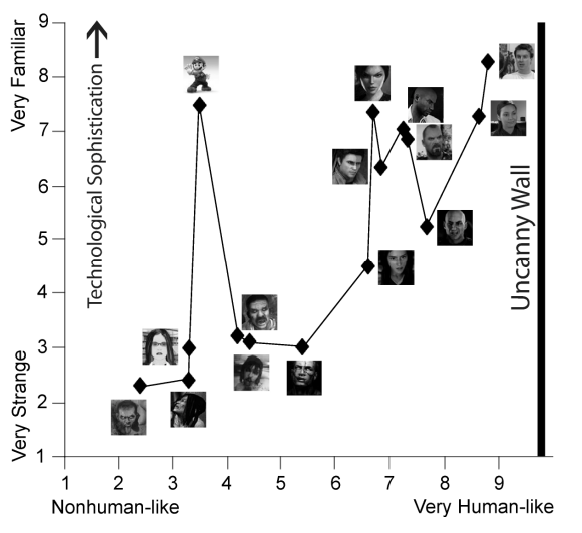
\includegraphics[width=0.5\textwidth]{graphics/uncanny_wall_graph.png}
    \caption{Hypothesized uncanny wall.}
    \label{fig:uncannyWallGraph}
\end{wrapfigure}
As seen from the constructed graph \ref{fig:uncannyWallGraph}, there is no single valley to be found.
It can therefore be assume that the uncanny valley lacks the clarity proposed by Masahiro Mori and paints a more difficult picture with multiple influences affecting the familiarity towards humanlike entities felt by participants. The fact that no virtual character could outperform a real person, even though all participants were previously exposed to the effects of the uncanny valley in their everyday lives, this study suggests that the uncanny valley can be better defined by an uncanny wall. Therefore it may be not possible to traverse the uncanny valley defined by Masahiro Mori. Furthermore the study assumes that with the factor of time audiences do not get used to the uncanny valley effect but that time leads to an increasing discernment on the part of viewers to more small details which do not perfectly resemble real humans. Through this sophistication of discernment the uncanny wall rises with time.\\
This study thus paints a new picture of the uncanny valley in which it is not possible to overcome it, even with ever-improving technological possibilities. However, it is also worth mentioning that the study's statements should be again validated by conducting the study again with the new possibilities in the development of humanlike designs which have emerged in recent times. In such a repeated study, a larger number of participants should be chosen, who are not all familiar with the subject matter. Finally, when selecting the characters, care should be taken that they are not known to the participants to not influence the ratings of the participants.







